\chapter{Cluster analysis}


Finding groups of objects such that the objects in a group
will be similar (or related) to one another and different
from (or unrelated to) the objects in other groups.

The aim of clustering is to ease data \textbf{understanding} and \textbf{summarization}, i.e. reduce the size of data sets.

\note{
	The following are \textit{NOT} cluster analysis:
	\begin{itemize}
		\item Simple segmentation
		\begin{itemize}
			\item Dividing students into different registration groups
		\end{itemize}
		alphabetically, by last name
		\item Results of a query
		      \begin{itemize}
			      \item Groupings are a result of an external specification
			      \item Clustering is a grouping of objects based on the data
		      \end{itemize}
		\item Supervised classification
		      \begin{itemize}
			      \item Have class label information
		      \end{itemize}
		\item Association Analysis
		      \begin{itemize}
			      \item Local vs. global connections
		      \end{itemize}
	\end{itemize}

	These ain't clustering essentially because there is no \textbf{similarity} measure involved, which instead is the core of clustering.
}

\begin{figure}[htbp]
   \centering
   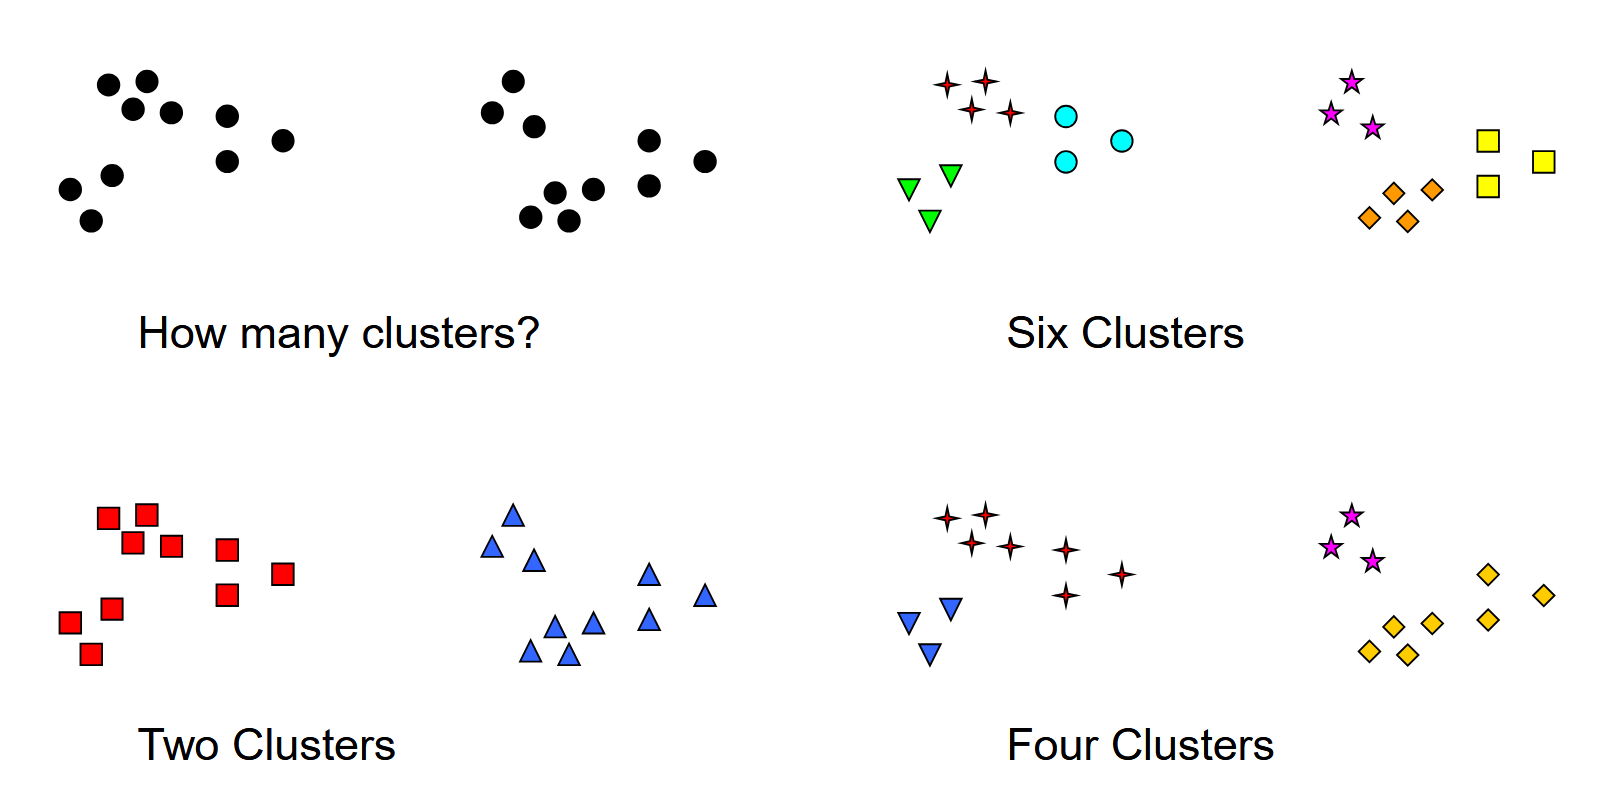
\includegraphics{images/04/clustering.png}
   \caption{``Cluster'' may be an amibguous term. How to define a cluster? How big is a cluster? How many clusters are there?}
   \label{fig:04/clustering}
\end{figure}

\section{Definitions}
A \textbf{clustering} is a set of clusters. There is an important distinction between hierarchical and
partitional sets of clusters.
\begin{itemize}
	\item \textit{Partitional} Clustering\\
	A division of data objects into non-overlapping subsets
	(clusters) such that each data object is in exactly one subset.
	\item \textit{Hierarchical} Clustering\\
	A set of nested clusters organized as a hierarchical tree.
\end{itemize}

\begin{figure}[htbp]
	\centering
	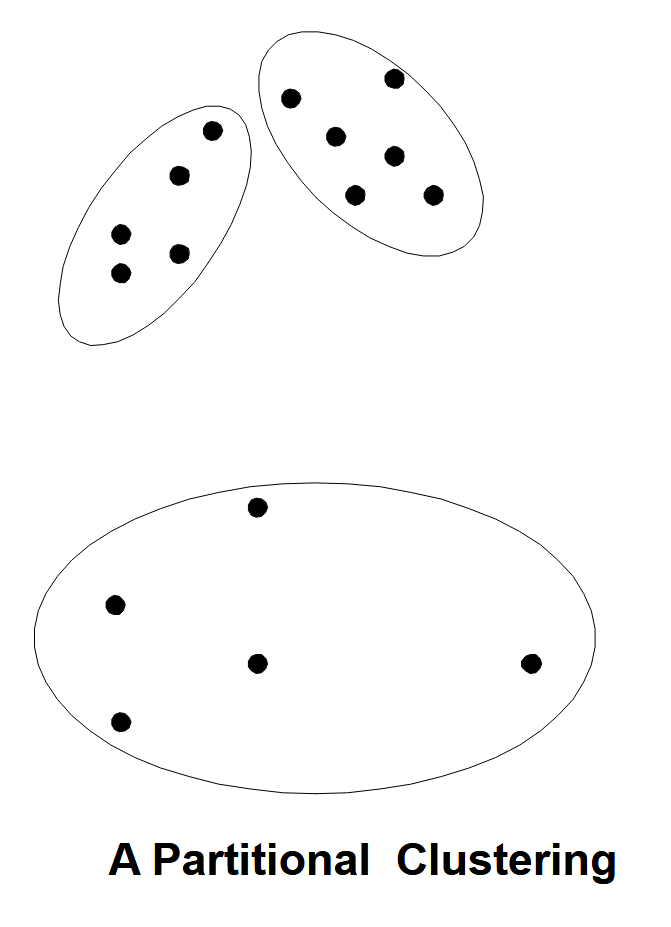
\includegraphics[width=0.33\columnwidth]{images/04/partitional.png}
	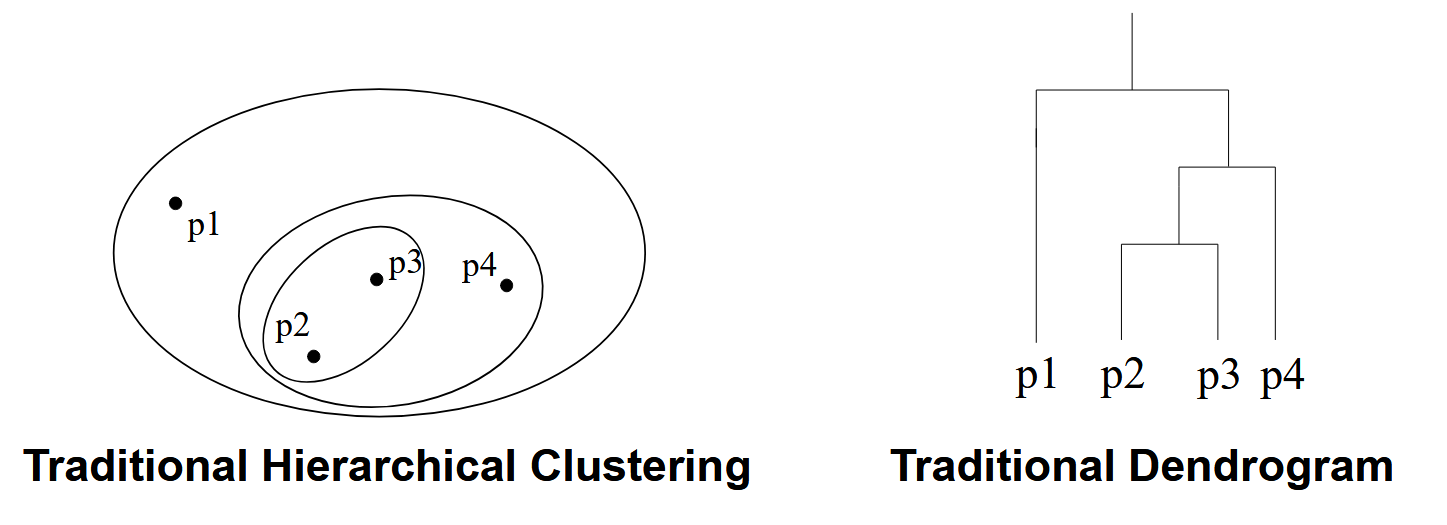
\includegraphics[width=0.66\columnwidth]{images/04/hierarchical.png}
	\caption{Partitional vs Hierarchical clustering}
	\label{fig:04/partitional_hierarchical}
\end{figure}


There are other distinctions among clusterings:
\begin{itemize}
	\item Exclusive versus non-exclusive
	      \begin{itemize}
		      \item In non-exclusive clusterings, points may belong to multiple
	      \end{itemize}
	      clusters.
	      \begin{itemize}
		      \item Can represent multiple classes or ‘border’ points
	      \end{itemize}
	\item Fuzzy versus non-fuzzy
	      \begin{itemize}
		      \item In fuzzy clustering, a point belongs to every cluster with some
		            weight between 0 and 1
		      \item Weights must sum to 1
		      \item Probabilistic clustering has similar characteristics
	      \end{itemize}
	\item Partial versus complete
	      \begin{itemize}
		      \item In some cases, we only want to cluster some of the data
	      \end{itemize}
	\item Heterogeneous versus homogeneous
	      \begin{itemize}
		      \item Clusters of widely different sizes, shapes, and densities
	      \end{itemize}
\end{itemize}

\section{Types of Clustering}
% // TODO add pictures
\begin{itemize}
	\item Well-separated clusters
	A cluster is a set of points such that any point in a cluster is closer (or more similar) to every other point in the cluster than to any point not in the cluster
	\item Center-based clusters
	\begin{itemize}
		\item A cluster is a set of objects such that an object in a cluster is
closer (more similar) to the “center” of a cluster, than to the
center of any other cluster
	\item The center of a cluster is often a centroid, the average of all
the points in the cluster, or a medoid, the most “representative”
point of a cluster
	\end{itemize}
	\item Contiguous clusters (Nearest neighbor or
Transitive)
\begin{itemize}
	\item Each point is closer to at least one point in its cluster than to
any point in another cluster.
	\item Graph based clustering
	\item This approach can have trouble when noise is present since a
small bridge of points can merge two distinct clusters
\end{itemize}
	\item Density-based clusters
	\begin{itemize}
		\item A cluster is a dense region of points, which is separated by
low-density regions, from other regions of high density.
	\item Used when the clusters are irregular or intertwined, and when
noise and outliers are present.
\item Points which are not classfied as part of any cluster are considered noise. In the figure they may be the gray blackground points.
	\end{itemize}
	\item Property or Conceptual
	\item Described by an Objective Function
\begin{itemize}
	\item Finds clusters that minimize or maximize an objective
function.
	\item Enumerate all possible ways of dividing the points into
clusters and evaluate the `goodness' of each potential
set of clusters by using the given objective function.
	\item NP Hard)
	\item Can have global or local objectives.
	\begin{itemize}
		\item Hierarchical clustering algorithms typically have local objectives
		\item Partitional algorithms typically have global objectives
	\end{itemize}
\end{itemize}
\end{itemize}

\newpage
\section{Similarity}
\begin{itemize}
    \item Similarity
          \begin{itemize}
              \item Numerical measure of how alike two data objects are.
              \item Is higher when objects are more alike.
              \item Often falls in the range [0,1]
          \end{itemize}
    \item Dissimilarity
          \begin{itemize}
              \item Numerical measure of how different are two data objects
              \item Lower when objects are more alike
              \item Minimum dissimilarity is often 0
              \item Upper limit varies
          \end{itemize}
    \item Proximity refers to a similarity or dissimilarity
\end{itemize}

\subsection{Euclidean Distance}
The most common way to measure distance between two data objects is the Euclidean distance:

\[
d(\mathbf{x}, \mathbf{y}) = \sqrt{\sum_{k=1}^{n}(x_k - y_k)^2}
\]

where $n$ is the number of dimensions (attributes) and $x_k$ and $y_k$ are, respectively, the $k^{th}$ attributes (components) or data objects $\mathbf{x}$ and $\mathbf{y}$. Standardization is necessary, if scales differ.

\begin{itemize}
    \item Standardization is necessary, if scales differ.
\end{itemize}

\subsection{Similarity and Dissimilarity for Different Attribute Types}

% \begin{table}[htbp]
% \centering
% \caption{Similarity and dissimilarity for simple attributes}
% \begin{tabular}{|p{3cm}|p{6cm}|p{4cm}|}
% \hline
% \textbf{Attribute Type} & \textbf{Dissimilarity} & \textbf{Similarity} \\
% \hline
% Nominal & 
% $d = \begin{cases}
% 0 & \text{if } p = q \\
% 1 & \text{if } p \neq q
% \end{cases}$ & 
% $s = \begin{cases}
% 1 & \text{if } p = q \\
% 0 & \text{if } p \neq q
% \end{cases}$ \\
% \hline
% Ordinal & 
% $d = \frac{|p-q|}{n-1}$

% (values mapped to integers 0 to $n-1$, where $n$ is the number of values) & 
% $s = 1 - \frac{|p-q|}{n-1}$ \\
% \hline
% Interval or Ratio & 
% $d = |p - q|$ & 
% $s = -d$, $s = \frac{1}{1+d}$ or

% $s = 1 - \frac{d-min\_d}{max\_d-min\_d}$ \\
% \hline
% \end{tabular}
% \label{tab:similarity_attributes}
% \end{table}

% $p$ and $q$ are the attribute values for two data objects.

\subsubsection{Minkowski Distance}

Minkowski Distance is a generalization of Euclidean Distance. $r$ is a parameter that defines the type of distance, $n$ is the number of dimensions (attributes) and $x_k$ and $y_k$ are, respectively, the $k^{th}$ attributes (components) or data objects $\mathbf{x}$ and $\mathbf{y}$.

\[
d(\mathbf{x}, \mathbf{y}) = \left(\sum_{k=1}^{n} |x_k - y_k|^r\right)^{\frac{1}{r}}
\]

\begin{itemize}
	\item For $r=1$, it is the Manhattan distance (or city block/Hamming distance)
	\item For $r=2$, it is the Euclidean distance
	\item For $r \rightarrow \infty$, it is the supremum distance (or Chebyshev distance)
\end{itemize}

%  // TODO

\section{K-Means}
\begin{itemize}
	\item Partitional clustering approach
	\item Number of clusters, K, must be specified
	\item Each cluster is associated with a centroid (center point)
	\item Each point is assigned to the cluster with the closest
centroid
	\item The basic algorithm is very simple
\end{itemize}